\documentclass[10pt,twocolumn]{article}
\usepackage[margin=0.75in,columnsep=0.28in]{geometry}
\usepackage{times}
\usepackage{natbib}
\usepackage{graphicx}
\usepackage{booktabs}
\usepackage{amsmath}
\usepackage{hyperref}
\usepackage{caption}
\setlength{\bibsep}{1pt}

\title{\Large Does the Voice Change the Grade?\\[2pt]
\large A Causal Audit of Speaker-Identity Bias\\in Audio-LLM Judges}
\author{Mohammed Abraar \\ \small Vizuara Research \\ \small \texttt{abraar@vizz.vizuara.ai}}
\date{}

\begin{document}
\maketitle

\begin{abstract}
Audio language models now grade spoken answers directly: automated oral exams,
AI interview screening, and speech leaderboards all use an audio-input model
as the judge. Every one of these systems assumes the judge scores what was
said, not how it sounded. We test that assumption. We hold a bank of 24
interview-style answers fixed and render each one in four accents (American,
British, Indian, and Nigerian English) and two speaker genders using
text-to-speech, then score every clip with two audio-input judges, Gemini 3.1
Pro and Gemini 3.6 Flash, one clip per call, temperature zero, blind to the
purpose of the study. First, Gemini 3.1 Pro scores Indian-accented answers 2.5
points lower than the identical answer in an American accent, on a 0 to 100
scale (95\% CI $-4.06$ to $-0.94$, $p=0.005$, $d_z=-0.44$). Second, Gemini 3.6
Flash shows no such penalty on the same comparison (mean shift $-0.04$,
$p=1.0$): two models from the same company, hearing the identical audio,
disagree about whether an accent lowers the score. Third, a decomposition arm
traces the Gemini 3.1 Pro penalty to the acoustic channel. Grading from the
model's own transcript of the same audio erases the effect (mean shift
$+1.88$, $p=0.14$), and grading from the frozen gold transcript also erases it
($-0.83$, $p=0.51$). Fourth, we test five delivery perturbations, filled
pauses, faster or slower speech, an 8kHz telephone codec, and background
noise, and find no significant score shift under either judge at this sample
size, a result we read as inconclusive given the sample rather than as
evidence that delivery never leaks into the score. We pre-registered the
direction of the accent effect before collecting data, and we also find a
partial reversal: Nigerian-accented answers trend toward higher scores under
both judges, the opposite of the predicted direction. We report it as we
found it.
\end{abstract}

\section{Introduction}

An audio language model that grades a spoken answer is being asked to do two
things at once: understand the content, and ignore everything about the
voice that carries it. Three deployed systems already depend on that second,
unstated assumption holding. Automated oral-language assessment tools grade
non-native speakers on scales that claim to measure content, not accent
\citep{ma2025assessmentof}. AI interview-screening pipelines already
process hundreds of thousands of real candidate interviews with an
LLM-as-judge step in the loop \citep{allbert2025evaluatingsp}, on top of a
pre-LLM fairness literature that already catalogued bias sources in
automated video interviews \citep{booth2023integratingp}. Speech
leaderboards increasingly use an audio-capable model, rather than a human
panel, to rank system outputs \citep{manakul2025audiojudgeun}. None of these
deployments has been checked against the one manipulation that would prove
or disprove the assumption directly: holding what is said perfectly fixed,
and changing only who appears to be saying it.

We run that check. We author a bank of 24 short spoken answers once, freeze
the text, and render each answer in four accents and two speaker genders
using text-to-speech, so that every clip in a comparison carries the
identical words. We then have two audio-input judges, Gemini 3.1 Pro and
Gemini 3.6 Flash, score every clip on a 0 to 100 rubric, one clip per call,
never told that the study concerns voice. Because the text is identical by
construction, any score difference between two renderings of the same item
can only be explained by the voice.

This paper makes four contributions.
\begin{enumerate}
\item A causal audit that puts an audio-input language model in the grader
role and varies the evaluee's own accent and gender while holding the
answer's content fixed (Section~\ref{sec:method}).
\item A decomposition design that separates acoustic-channel bias from
transcription-channel bias by grading the same item three ways: end-to-end
audio, the judge's own transcript of that audio, and the frozen gold
transcript (Section~\ref{sec:decomp}).
\item A judge-family comparison showing that two models from the same
company can disagree about whether an accent changes the score of identical
content, one showing a significant penalty and the other showing none
(Section~\ref{sec:results}).
\item A delivery-perturbation battery, filled pauses, speaking rate,
telephone-bandwidth audio, and background noise, tested under both a neutral
rubric and an explicit instruction to ignore delivery
(Section~\ref{sec:delivery}).
\end{enumerate}

\section{What Was Known and What Is New}

The premise that audio-language-model judges carry biases is not new. What
is new is which bias, and in which role.

\textbf{AudioJudge} \citep{manakul2025audiojudgeun} establishes that
large audio models can act as judges of speech, and catalogs verbosity and
position bias in that role. It never varies the identity of the speaker
being judged; its evaluees are text-to-speech systems, not people.

\textbf{The Voice Behind the Words} \citep{satish2026thevoicebehi}, and its
companion study using the same cohort and an explicitly judge-free protocol
\citep{satish2026fromseeingit}, are the closest papers by topic. It varies the accent and gender of a
\emph{question-asker} across 2,880 controlled interactions and finds that a
SpeechLLM's own reply is rated less helpful for some accents. But the judge
in that paper is explicitly text-only and voice-blind: it reads only the
assistant's written reply, never the audio. Voice never reaches the judge in
that design. It cannot show, and does not claim, that an audio-input judge's
score of an evaluee's own answer moves with that evaluee's voice, which is
the exact question this paper asks.

\textbf{BiasInEar} \citep{wei2026biasintheear} varies the voice of a spoken
multiple-choice question and measures whether the model's own answer choice
changes. The model here is the test-taker, not a judge; there is no evaluee
and no score assigned to anyone's spoken answer.

\textbf{ParaPairAudioBench} \citep{jeon2026parapairaudi} puts an audio
model in the judge role and tests whether it can correctly detect and rank
paralinguistic differences such as gender and age. That is the inverse of
our question: it asks whether the judge notices the attribute when told to
look for it, not whether the attribute leaks into an unrelated content
score when the judge is not told to look for it at all.

\textbf{Bias Analysis of L2 Speaking Assessment Systems}
\citep{labroo2026biasanalysis} audits a real speaking-assessment grader for
encoded speaker attributes, but the audit is representational, probing
internal activations on naturally varying speakers, not a controlled
same-content voice swap.

What remains uncovered by all of the above, and is the subject of this
paper, is the exact intersection: an audio-input model in the grader role,
the evaluee's own voice identity as a randomized treatment, and a content
score as the outcome, with the text held identical across every condition.

Three further clusters of recent work sit adjacent to this gap without
closing it. A judge-construction literature builds and validates audio
judges without a bias axis at all
\citep{wang2025speechllmasj,zhang2026jastinaligni,chen2025audiolargela,
manakul2025audiojudgeun,park2026auditingprot}, including judges of speaking
style \citep{chiang2025audioawarela} and disfluency robustness of
comprehension rather than of scoring
\citep{liu2025vocalbenchdf,takagi2026investigatin}. An advisor-role and
assistant-role literature varies a user's paralinguistics and measures the
model's own generated response, decision, or recommendation, not a grade
assigned to the user's speech
\citep{wu2025evaluatingbi,lin2026vibevoiceind,satish2025speakyourmin,
satish2025dobiasbenchm,choi2025acousticbase}. A deployed-assessment
literature grades real L2 speech but audits fairness observationally across
naturally different speakers rather than through a controlled voice swap on
identical content
\citep{uehara2026interpretabl,ginjala2026doLLMdecoders,koenecke2020racial}.
None of these fifteen papers manipulates an evaluee's accent or gender as a
randomized treatment on a content score. \citet{miller2026doaudiolangu}
comes closest procedurally, holding a transcript fixed while varying affect
and prosody to test whether a judge uses audio evidence at all, but the
manipulated factor is delivery, not demographic identity, and the outcome is
evidence-use correctness rather than a bias in the assigned score.

Two literatures we deliberately stay out of. Voice-agent jailbreak and
refusal work studies how prosody and emotion bypass safety training, a
different outcome variable than a content grade
\citep{jain2025voiceagentbench}. TTS-instrument validity work, on accent
fidelity \citep{zhong2025pairwiseeval,huang2026codecmosacce,
xinyuan2025scalablecont}, on the reliability of TTS-as-stimulus methodology
\citep{yang2025positiontowa}, and on MOS-annotator demographics
\citep{ren2026mosbiasfromh}, informs our manipulation-check design but does
not audit a judge. We also note \citet{tam2025medvoicebias}, which finds
large modality-driven shifts in a different deployed setting, clinical
recommendation, using synthetic voices without an accent axis, and
\citet{wang2026priorongevidence}, which uses the same real-speech corpus we
plan as our causal anchor for a diagnostic-feedback task rather than a
content-grading one. The human-listener precedent for our exact design
predates audio language models entirely: \citet{kang2009reverse} show that
identical recorded speech is rated less comprehensible when paired with a
different apparent speaker identity, the same causal logic we apply here to
an artificial judge instead of a human one.

\textbf{Significance.} If a judge's score of a spoken answer depends on the
speaker's accent, every deployed pipeline listed in the introduction is
partly scoring the speaker rather than the answer. The practical
consequence we test directly is whether the standard proposed fix, grading
from a transcript instead of from audio, actually removes the effect. Our
decomposition arm answers that question for the one bias we find: yes, for
that judge, on that accent.

\section{Method}
\label{sec:method}

\subsection{Answer Bank}

We authored 24 interview-style question-and-answer pairs across ten everyday
domains (science, history, cooking, health, technology, culture, geography,
personal finance, daily-life advice, and education), using a frozen text
model. Each answer targets a medium quality band, not a strong or a weak
one, because a judge has no room to move a score that is already near a
ceiling or a floor.

Our first attempt at this calibration failed, and we report the failure
because it changed our design. A prompt asking the model for a merely
``incomplete or shallow'' answer produced answers that a real audio judge
scored at a mean of 94.3 out of 100 (standard deviation 4.5, minimum 85), a
ceiling with no headroom for any bias to move the score. We diagnosed this
before collecting any of the results reported below, and rewrote the
generation prompt to require specific, checkable weaknesses in each answer:
answering only part of the question, hedging language, one clear factual
gap, and a weak ending. We validated the rewritten prompt on five test
answers scored by the real judge before regenerating the full bank; the
calibration answers scored 35, 35, 45, 60, and 65. The full 24-item bank
regenerated under this corrected prompt scored a mean of 61.3 (standard
deviation 17.0, range 20 to 90) under Gemini 3.6 Flash, the distribution
used throughout this paper.

\subsection{Accent and Gender Conditions (Axis A)}

Each of the 24 answers was rendered with \texttt{gemini-3.1-flash-tts-preview}
in four accents, American, British, Indian, and Nigerian English, crossed
with two voices (one designated male, one female), producing 192 clips. The
accent is specified as a natural-language style instruction to the TTS
model, together with a fixed voice choice per gender. We validated that the
TTS model actually renders the requested accent with an 8-clip manipulation
check before generating the study data: a separate blind classifier judge
correctly identified the intended accent and gender in 8 of 8 clips, all at
high stated confidence. Every clip was loudness-normalized
(\texttt{ffmpeg loudnorm}) and resampled to 16kHz.

\subsection{Delivery Conditions (Axis B)}

Using one fixed voice (the American-accented female condition), we
generated five delivery perturbations of each of the 24 answers: filled
pauses (``um,'' ``uh'' inserted at clause boundaries, re-synthesized by
TTS), a slowed and a sped-up rendering (\texttt{ffmpeg atempo} at 0.85 and
1.25), an 8kHz mu-law telephone-bandwidth rendering, and a background-noise
condition mixing synthesized pink noise at a measured 10dB
signal-to-noise ratio. We do not have a licensed multi-talker babble corpus,
so the noise condition uses a pink-noise proxy rather than authentic babble;
we state this as a limitation rather than presenting it as equivalent to a
babble-noise benchmark.

Every perturbed clip passed a word-error-rate neutrality check before being
judged: we transcribed each clip and compared it to the frozen source text,
excluding any clip whose transcript changed by more than 5\% word error
rate, since a perturbation that changes the recognized words is no longer a
pure delivery manipulation, the same principle behind channel-specific
robustness suites for text pipelines \citep{hu2026shouldwetype}. Our first
transcription pass used a
general-purpose instruction and produced an artificially high failure rate,
because the transcribing model, an LLM used as an ad hoc speech recognizer,
occasionally filled in unrelated caption-like text (video timestamps, a
fragment of an unrelated course syllabus) instead of transcribing difficult
audio, rather than mis-hearing the actual words. A stricter prompt that
explicitly forbade inventing content flipped 28 of 33 initial failures to
passing, confirming that most of the initial failures were an artifact of
the transcribing model, not of the audio. The final gate excluded 5 of 120
non-baseline conditions as genuine word-error-rate violations. Both prompt
arms, a neutral rubric and an explicit instruction to grade content and
ignore delivery, were run on the 139 surviving clips.

\subsection{Judges and Protocol}

Two judges scored every clip: \texttt{gemini-3.6-flash} and
\texttt{gemini-3.1-pro-preview}, both called directly through the API at
temperature zero, one clip per call, in randomized order, never informed
that the study concerns voice or accent. The rubric asks for a single 0 to
100 score covering correctness, completeness, helpfulness, and clarity,
plus a one-sentence reason, returned as a structured JSON object. We did not
use a third, open-weight judge or an OpenAI judge in this draft; both remain
planned additions, discussed in Section~\ref{sec:limitations}.

\subsection{Decomposition Arm}
\label{sec:decomp}

For a stratified subset of Axis A, the American and Indian accents crossed
with both genders across 12 of the 24 items, we graded the same content
three ways per judge: end-to-end audio (already collected in Axis A), the
judge's own transcript of that same audio, and the frozen gold text
transcript. If a bias found in the audio mode shrinks under the transcript
modes, that localizes the bias in the acoustic channel rather than in the
model's general treatment of the content.

\subsection{Analysis}

The unit of analysis is the within-item score difference between a
treatment condition and a reference condition (the American-accent
rendering of the same gender for Axis A, the clean baseline for Axis B),
computed separately per judge and per condition. We report the mean shift
with a bootstrap 95\% confidence interval (10,000 resamples), a two-sided
sign-flip permutation test ($p$, 20,000 permutations), and the paired effect
size $d_z$. Every number in Section~\ref{sec:results} is read directly from
one scripted analysis pass over the raw judgment logs.

\section{Results}
\label{sec:results}

\subsection{Accent and Gender (Axis A)}

Table~\ref{tab:axisa} and Figure~\ref{fig:forest} report the score shift for
each non-American accent relative to the American-accent rendering of the
same item and the same gender, so the comparison is never confounded by
gender. Gemini 3.1 Pro shows one shift that clears our significance
threshold: Indian-accented answers score 2.5 points lower than the
identical American-accented answer ($p=0.005$, $d_z=-0.44$). The same
comparison under Gemini 3.6 Flash is indistinguishable from zero
($-0.04$, $p=1.0$). Neither judge shows a significant British-accent effect.
Both judges show a Nigerian-accent shift in the positive direction, the
opposite of our pre-registered prediction that global-South accents would
score lower; neither reaches significance at this sample size. The gender
main effect (female minus male, within the American-accent condition) is
not significant for either judge, though Gemini 3.6 Flash trends toward
scoring the female voice 3.25 points higher ($p=0.12$).

\begin{table}[t]
\centering
\small
\caption{Score shift, non-American accent minus American accent, same item
and gender ($n=48$ paired comparisons per cell). Bold marks $p<0.01$.}
\label{tab:axisa}
\begin{tabular}{lrrr}
\toprule
Accent & Mean shift & 95\% CI & $p$ \\
\midrule
\multicolumn{4}{l}{\emph{Gemini 3.1 Pro}} \\
UK      & $-0.42$ & [$-2.08$, $1.25$]  & 0.73 \\
Indian  & \textbf{$-2.50$} & [$-4.06$, $-0.94$] & \textbf{0.005} \\
Nigerian& $+1.04$ & [$-0.52$, $2.60$]  & 0.26 \\
\midrule
\multicolumn{4}{l}{\emph{Gemini 3.6 Flash}} \\
UK      & $-1.08$ & [$-3.90$, $1.92$]  & 0.49 \\
Indian  & $-0.04$ & [$-2.85$, $2.73$]  & 1.00 \\
Nigerian& $+0.23$ & [$-2.60$, $3.08$]  & 0.89 \\
\bottomrule
\end{tabular}
\end{table}

\begin{figure}[t]
\centering
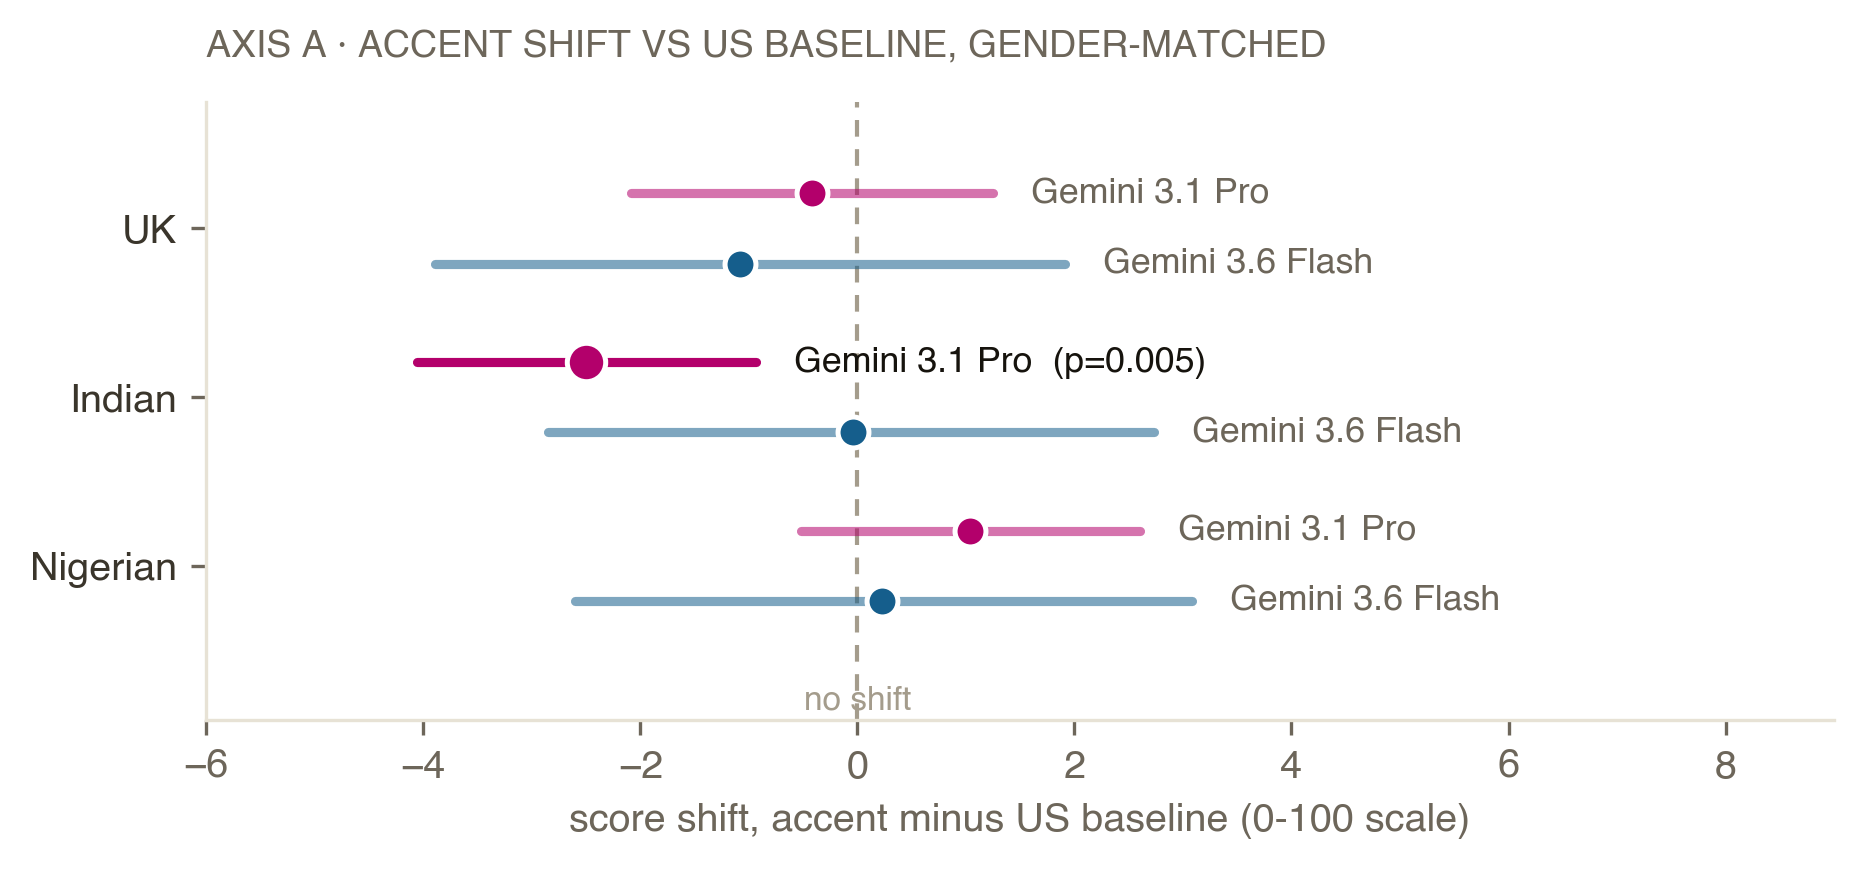
\includegraphics[width=\linewidth]{../figures/figure1_accent_forest.png}
\caption{Score shift by accent and judge, 95\% bootstrap confidence
intervals, $n=48$ paired comparisons per interval. Right of the dashed line
means the accent scored higher than the American baseline. Only the Gemini
3.1 Pro, Indian-accent interval (highlighted) excludes zero at $p<0.01$.}
\label{fig:forest}
\end{figure}

\subsection{Decomposition: Where the Bias Lives}

Table~\ref{tab:decomp} traces the Gemini 3.1 Pro Indian-accent penalty across
grading modes. The penalty is present and significant when the judge hears
audio ($-2.50$, $p=0.006$), reverses in sign and loses significance when the
judge grades its own transcript of the identical audio ($+1.88$, $p=0.14$),
and is not significant when the judge grades the frozen gold transcript
($-0.83$, $p=0.51$). This pattern is consistent with the bias living in the
acoustic channel specifically, not in a general dispreference for the
content once the accent is described in words. Gemini 3.6 Flash, which
showed no significant audio-mode effect to begin with, shows a
non-significant shift under its own transcript ($-4.25$, $p=0.17$) and under
the gold transcript ($+0.83$, $p=0.36$); we do not read a channel story into
a judge that showed no effect to decompose.

\begin{table}[t]
\centering
\small
\caption{Decomposition of the Indian-accent shift by grading mode, Gemini
3.1 Pro, $n=24$ paired comparisons per mode.}
\label{tab:decomp}
\begin{tabular}{lrrr}
\toprule
Mode & Mean shift & 95\% CI & $p$ \\
\midrule
Audio            & \textbf{$-2.50$} & [$-4.06$, $-0.94$] & \textbf{0.006} \\
Own transcript   & $+1.88$ & [$0.00$, $3.96$]   & 0.14 \\
Gold transcript  & $-0.83$ & [$-2.50$, $0.83$]  & 0.51 \\
\bottomrule
\end{tabular}
\end{table}

\subsection{Delivery (Axis B)}
\label{sec:delivery}

None of the five delivery perturbations produced a significant score shift
under either judge, under either the neutral rubric or the explicit
ignore-delivery instruction (all $p>0.1$; per-condition $n$ ranges from 21
to 24 after the word-error-rate exclusions). Effect sizes were small
throughout ($|d_z|<0.36$). We read this as inconclusive at the current
sample size rather than as evidence that delivery never affects content
scores: our own budget-driven power analysis at the planning stage flagged
that 24 items would leave wide intervals on the secondary axis, and the
observed intervals here span both directions of zero in every cell.

\section{Limitations}
\label{sec:limitations}

\textbf{Sample size.} The accent and delivery arms use 24 items under a
\$20 compute budget, smaller than the 150-item design of the predecessor
study this method is adapted from. The Indian-accent effect we report
survives that sample size; the null results on the delivery arm and on the
British and Nigerian accents may simply be underpowered.

\textbf{Two judge families, both from one company.} Every scored clip was
graded by Gemini 3.1 Pro or Gemini 3.6 Flash. We did not have access to an
OpenAI audio judge at the time of this draft, and had not yet completed the
integration of an open-weight audio judge on Modal. The disagreement between
two Gemini models is itself informative, since it shows the effect is not a
fixed property of one vendor's audio pipeline, but a genuine third-family
and fourth-family comparison remains future work.

\textbf{Text-to-speech only, no real-speech anchor yet.} Every accent
condition in this draft is synthetic. The L2-ARCTIC corpus
\citep{zhao2018l2arctic}, real recordings
of non-native English speakers reading identical prompts against matched
native recordings, is the planned causal anchor for this project, verified
for license and sentence-overlap suitability, but its use here is pending a
manual, human-completed registration step with the corpus's distributor
that had not finished at the time of this draft.

\textbf{Same-family manipulation check.} The 8-clip accent-fidelity check
used a Gemini model to classify audio generated by a different Gemini
model. The classification clips differ in content from the study items, but
a same-vendor circularity concern remains until an independent or
human-listener check is run.

\textbf{The noise condition is a proxy.} We synthesized pink noise at a
measured signal-to-noise ratio rather than mixing in a licensed
multi-talker babble corpus; a real babble condition may behave differently.

\section{Conclusion}

We asked a narrow question with a clean design: if the words are identical,
does an audio-input judge's score still move with the speaker's voice? For
one judge, Gemini 3.1 Pro, on one accent, Indian English, the answer is yes,
by 2.5 points on a 100-point scale, and the effect traces to the acoustic
channel rather than to the content once transcribed. For a sibling model
from the same company, Gemini 3.6 Flash, the answer on the identical
comparison is no. Both facts matter for anyone deploying an audio-LLM judge
today: which model you pick is not a neutral engineering choice, and
grading from a transcript is a concrete, tested mitigation for at least the
one failure mode we found. The delivery axis, the real-speech anchor, a
third judge family, and a prompt-level mitigation battery are the natural
next steps, and are already scoped in this project's experiment plan.

\bibliographystyle{plainnat}
\bibliography{refs}

\end{document}
